
\documentclass[a4,10pt]{ctexart}

\usepackage{ctex}
\usepackage[utf8]{inputenc}
\usepackage{amsfonts,amsmath,amscd,amssymb,amsthm}
\usepackage{latexsym,bm}
\usepackage{cite}
\usepackage{mathtools,mathdots,graphicx,array}
\usepackage{fancyhdr}
\usepackage{lastpage}
\usepackage{color}
\usepackage{enumitem}
\usepackage{mpdoc}
\usepackage{diagbox}
\usepackage{xcolor,tcolorbox,tikz,tkz-tab,mdframed,tikz-cd}
\usepackage{framed}
\usepackage{verbatim}
\usepackage{extarrows}
\usepackage{fontspec}
\newcommand*{\dif}{\mathop{}\!\mathrm{d}}
\newcommand*{\arsinh}{\mathop{}\!\mathrm{arsinh}}
\newcommand*{\artanh}{\mathop{}\!\mathrm{artanh}}
\newcommand*{\arcosh}{\mathop{}\!\mathrm{arcosh}}
\newcommand*{\Li}{\mathop{}\!\textrm{Li}}



\begin{document}
\pagenumbering{roman}
\title{随机过程课程作业-\textbf{Week3}}
\author{56-丁力-202328015926048}
\date{\today}
\maketitle
\tableofcontents
\newpage
\pagenumbering{arabic}
\newpage

\section{随机过程及其分类}

\begin{ti}{5}{}

    设二维随机变量 $(X, Y)$ 的联合密度函数为
    $$
    f(x, y)=\left\{\begin{array}{lc}
    \frac{4}{7}(1+y+x y), & 0<x<1,0<y<1 \\
    0, & \text { 其它 }
    \end{array}\right.
    $$
    试求随机变量 $Y(1+X)$ 的密度函数。
\end{ti}
    \begin{qj}\end{qj}

   
    % 在此处填写答案
    
    首先,我们需要找到满足 $z = y(1+x)$ 的 $(x,y)$ 对的范围。

    对于随机变量 $(X, Y)$ 的取值范围,我们可以将其分为两个区域。在区域A中,$y$ 的取值范围是 $(0, 1)$,而 $x$ 的取值范围是 $(0, z-1)$。在区域B中,$y$ 的取值范围是 $(0, \frac{z}{x+1})$,而 $x$ 的取值范围是 $(z-1, 1)$。

    
    接下来,我们可以分别对这两个区域进行积分。
    首先,我们考虑区域A的积分:
    $$
    g_A(z) = \int_{0}^{z-1} \int_{0}^{1} \frac{4}{7}(1+y+xy) , dy , dx
    $$
    
    然后,我们考虑区域B的积分:
    $$
    g_B(z) = \int_{z-1}^{1} \int_{0}^{\frac{z}{x+1}} \frac{4}{7}(1+y+xy) , dy , dx
    $$
    
    经过计算,我们得到区域A的积分 $g_A(z)$ 为:
    $$
    g_A(z) = \frac{6(-1 + z)}{7} + \frac{(-1 + z)^2}{7}
    $$
    
    区域B的积分 $g_B(z)$ 为:
    $$
    g_B(z) = \frac{-2z(2+z)\ln\left(\frac{z}{2}\right)}{7}
    $$
    
    因此,总的分布函数 $g(z)$ 为:
    $$
    g(z) = \frac{-5 + 4z + z^2 - 2z(2 + z)\ln\left(\frac{z}{2}\right)}{7}
    $$
    


    
    \begin{ti}{6}{}

        设 $X_1, X_2 , X_3$ 为独立同分布的随机变量, 且服从标准正态分布。令:
        $$
        Y=\frac{X_1+X_2 X_3}{\sqrt{1+X_3^2}}
        $$
        (a)试求随机变量 $Y$ 的分布密度函数;
        (b)试问有限个独立正态分布随机变量经过非线性变换是否可以服从正态分布?
    
\end{ti}
    \begin{proof}

    \end{proof}
  
    \begin{ti}{7}{}

       设 $\left\{\xi_n, n \geq 1\right\}$ 为独立同分布连续型随机变量序列, 令:
        $$
        \tau=\min \left\{n: n \geq 2, \xi_n>\xi_1\right\}, \sigma=\min \left\{n: n>m, \xi_n>\max _{1 \leq k \leq m}\left\{\xi_k\right\}\right\}
        $$
        试回答以下问题:
        (a) 求随机变量 $\tau$ 的分布函数, 并确定随机变量 $\tau$ 的数学期望是否存在;
        (b) 求概率 $P\{\sigma>n\}(n \geq m+1)$ 。
        

\end{ti}

\begin{qj}

\end{qj}


    
    \begin{ti}{8}{}

        设 $\xi_1, \xi_2, \cdots \xi_n$ 与 $\eta$ 为随机变量, $\eta \sim U[0,1]$, 而 $\xi_i(i=1,2, \cdots n)$ 均以下述条件概率取 1 和 0 两个, 即: $P\left\{\xi_i=1 \mid \eta=p\right\}=p, P\left\{\xi_i=0 \mid \eta=p\right\}=1-p$; 并且条件独立, 即对于 $i=1,2, \cdots, n$, 均有 $x_i=0,1$ 时, 有
        $$
        P\left\{\xi_1=x_1, \cdots, \xi_n=x_n \mid \eta\right\}=P\left\{\xi_1=x_1 \mid \eta\right\} \cdots P\left\{\xi_n=x_n \mid \eta\right\}
        $$
        试回答以下问题:
        (a) 试求 $P\left\{\xi_1=x_1, \cdots, \xi_n=x_n\right\}$;
        (b) 试求随机变量 $S_n=\xi_1+\cdots+\xi_n$ 的分布;
        (c) 试求条件分布 $P\left\{\eta \leq p \mid S_n=x\right\}$, 并求出密度函数, 其中: $x=x_1+\cdots x_n$;
        (d) 试问分布 $P\left\{\eta \leq p \mid S_n=x_1+\cdots x_n\right\}$ 与 $P\left\{\eta \leq p \mid \xi_1=x_1, \cdots, \xi_n=x_n\right\}$ 是否相 同, 其中: $p \in(0,1)$ 。


    \end{ti}

%     {

%     \centering
%     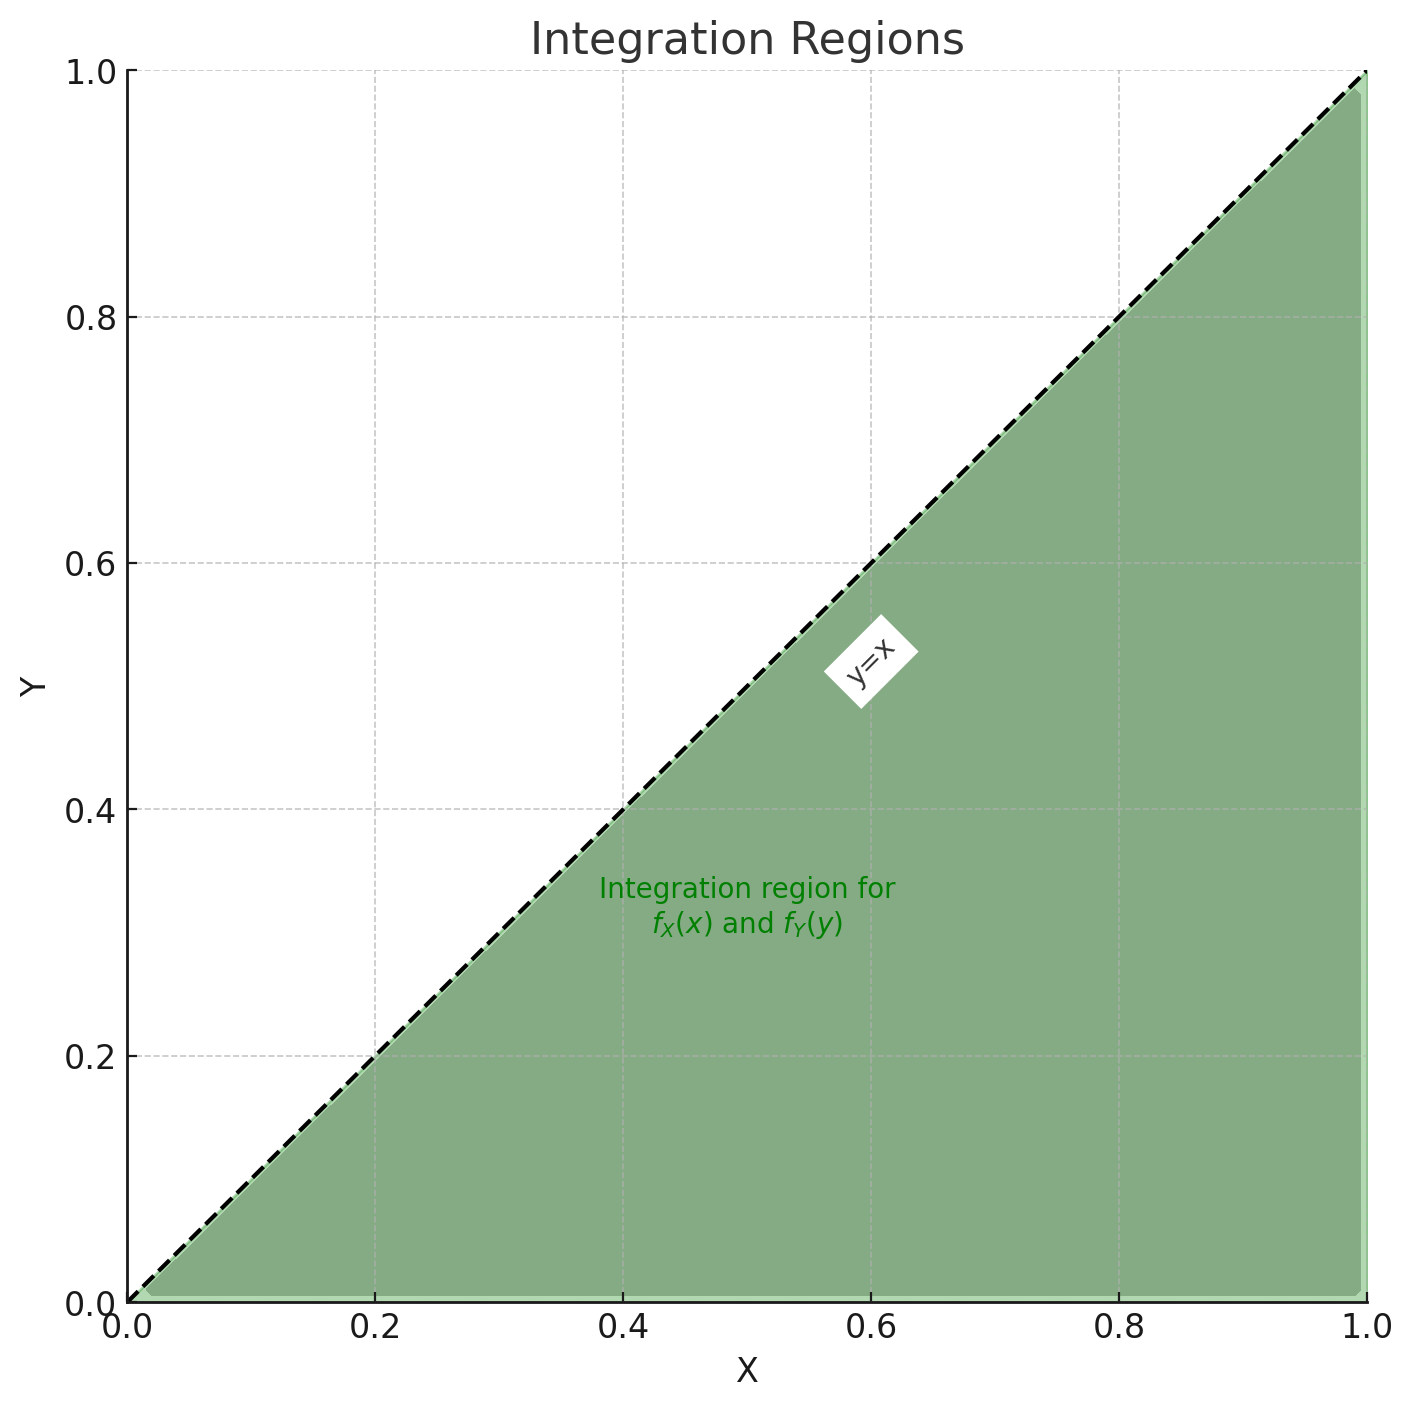
\includegraphics[scale=0.5]{images/1.png}
%     \par

% }

%     \begin{qj}
   
    


    
% \end{qj}

    

% \section{引言}

% 最近闲来无事, 整理了一个写文章看上去比较好用的模板. 

% 你可以对照源代码, 来看一下如何使用这些内容.

% 需要一定的基础. 

% \section{常用环境}
% \begin{yd}{这是一个约定}{}
              
% 约定的内容.
% \end{yd}

% 上述就是一些文本了. 使用的代码是
% \begin{lstlisting}{language=latex}
% \begin{yd}{这是一个约定}{}
              
% 约定的内容.
% \end{yd}
% \end{lstlisting}

% \begin{zs}
        
% 这是一个注释
    
% \end{zs}
    
% \begin{xt}
        
% 这是一个习题.
    
% \end{xt}
    
% \begin{lt}
        
% 这是一个问题.
    
% \end{lt}

% \begin{yl}
        
% 这是一个引理.
    
% \end{yl}

% \begin{dl}{A}{}
        
% 这是一个定理.
    
% \end{dl}
    
% \begin{tl}{A}{}
        
% 这是一个推论.
    
% \end{tl}

% \begin{dy}{A}{}
        
% 这是一个定义.
    
% \end{dy}

% \begin{jl}{A}{}
        
% 这是一个结论.
    
% \end{jl}

% \begin{mt}{A}{}
        
% 这是一个命题.
    
% \end{mt}

% \begin{ti}{A}{}
        
% 这是一个题目.
    
% \end{ti}

% \begin{cx}{A}{}
        
% 这是一个猜想.
    
% \end{cx}

% \begin{zy}
        
% 这是注意.
    
% \end{zy}

% \begin{ts}
        
% 这是一点提示.
    
% \end{ts}

% \begin{lt}
        
% 这是一个例题.
    
% \end{lt}

% \begin{proof}
% 你还可以加一点证明. 
% \end{proof}

% 我们注意到, 所有的数学公式将自动转换成行间公式的大小, 比如${1\over 2^k}$, $\sum_{i=0}^{998244353}i$. 

% \section{起源与未来的修改计划}

% 起源与hkmod的模板, 添加了一些常用的标志词. 可以在mpdoc.sty里面进行更改, 相信根据注释你也会. 

% 使用愉快! 
    
    
    
    
   

\end{document}
